\documentclass[11pt,letterpaper]{article}
\usepackage[T1]{fontenc}
\usepackage[scaled]{helvet}
\renewcommand{\familydefault}{\sfdefault}
\usepackage{amsmath,amssymb}
\usepackage[margin=0.8in,bottom=0.9in]{geometry}
\usepackage[most]{tcolorbox}
\usepackage{tikz}
\usetikzlibrary{calc}
\usepackage{enumitem}
\usepackage{array}
\usepackage{needspace}
\usepackage{fancyhdr}
\usepackage{pifont}

% ---- Palette "F. Bright & Playful" ----
\definecolor{fmtitle}{HTML}{3D2C8D}
\definecolor{fmkey}{HTML}{0096C7}
\definecolor{fmwatch}{HTML}{2BB673}
\definecolor{fmturn}{HTML}{F4A100}
\definecolor{fmmistake}{HTML}{EF476F}
\definecolor{fmnotice}{HTML}{9B5DE5}
\definecolor{fmgray}{HTML}{6B6B6B}

\pagestyle{fancy}
\fancyhf{}
\renewcommand{\headrulewidth}{0pt}
\fancyfoot[C]{\footnotesize\color{fmgray}\textcopyright\ 2026 FangMath. All rights reserved.}
\fancyfoot[R]{\footnotesize\color{fmgray}\thepage}
\setlength{\parindent}{0pt}
\setlength{\parskip}{3pt}

\newcommand{\badge}[1]{\colorbox{fmtitle}{\color{white}\bfseries\small\ #1\ }}
\newcommand{\leveltag}[2]{\colorbox{#1}{\color{white}\bfseries\scriptsize\ #2\ }}
\newcommand{\LE}{\leveltag{fmwatch}{EASY}}
\newcommand{\LM}{\leveltag{fmturn}{MEDIUM}}
\newcommand{\LH}{\leveltag{fmmistake}{HARD}}

\newcommand{\sectionbar}[2]{\needspace{6cm}\par\vspace{4mm}
  \begin{tcolorbox}[enhanced,colback=fmtitle,colframe=fmtitle,arc=2mm,
    left=4mm,top=1.5mm,bottom=1.5mm]
  \color{white}\bfseries\large #1\hfill{\normalsize\mdseries #2}
  \end{tcolorbox}}

\newtcolorbox{keyidea}{enhanced,breakable,colback=white,colframe=fmkey,boxrule=1pt,arc=2mm,
  title={Key Idea},coltitle=fmkey,fonttitle=\bfseries,
  attach boxed title to top left={xshift=4mm,yshift=-2mm},
  boxed title style={colback=white,colframe=fmkey,boxrule=0.9pt}}
\newtcolorbox{watchme}{enhanced,colback=white,colframe=fmwatch,boxrule=1pt,arc=2mm,
  title={Watch Me --- Worked Example},coltitle=fmwatch,fonttitle=\bfseries,
  attach boxed title to top left={xshift=4mm,yshift=-2mm},
  boxed title style={colback=white,colframe=fmwatch,boxrule=0.9pt}}
\newtcolorbox{mistakebox}{enhanced,breakable,colback=white,colframe=fmmistake,boxrule=1pt,arc=2mm,
  title={Common Mistake},coltitle=fmmistake,fonttitle=\bfseries,
  attach boxed title to top left={xshift=4mm,yshift=-2mm},
  boxed title style={colback=white,colframe=fmmistake,boxrule=0.9pt}}
\newtcolorbox{yourturn}{enhanced,breakable,colback=white,colframe=fmturn,boxrule=1pt,arc=2mm,
  title={Your Turn},coltitle=fmturn,fonttitle=\bfseries,
  attach boxed title to top left={xshift=4mm,yshift=-2mm},
  boxed title style={colback=white,colframe=fmturn,boxrule=0.9pt}}
\newtcolorbox{answerbox}[1]{enhanced,breakable,colback=white,colframe=fmwatch,boxrule=1pt,arc=2mm,
  title={#1},coltitle=fmwatch,fonttitle=\bfseries,
  attach boxed title to top left={xshift=4mm,yshift=-2mm},
  boxed title style={colback=white,colframe=fmwatch,boxrule=0.9pt}}

\newcommand{\work}[1]{\par\vspace{#1}}
\setlist[enumerate]{itemsep=2pt,topsep=3pt}

% ---------------- extra boxes ----------------
\newtcolorbox{notebox}{enhanced,breakable,colback=white,colframe=fmnotice,boxrule=1pt,arc=2mm,
  title={Notice},coltitle=fmnotice,fonttitle=\bfseries,
  attach boxed title to top left={xshift=4mm,yshift=-2mm},
  boxed title style={colback=white,colframe=fmnotice,boxrule=0.9pt}}
\newtcolorbox{exbox}{enhanced,colback=white,colframe=fmwatch,boxrule=0.8pt,arc=2mm,
  title={Example},coltitle=fmwatch,fonttitle=\bfseries\small,
  attach boxed title to top left={xshift=4mm,yshift=-2mm},
  boxed title style={colback=white,colframe=fmwatch,boxrule=0.8pt},fontupper=\small}
\newcommand{\topicbar}[1]{\needspace{4.5cm}\par\vspace{5mm}
  \begin{tcolorbox}[enhanced,colback=fmtitle,colframe=fmtitle,arc=2mm,left=4mm,top=1.5mm,bottom=1.5mm]
  \color{white}\bfseries\large #1
  \end{tcolorbox}}
\usepackage{multicol}

% ---------------- practice layout ----------------
\newcommand{\workline}{\par\vspace{7mm}{\color{gray!55}\rule{\linewidth}{0.4pt}}}
\newcommand{\worklines}[1]{\foreach \i in {1,...,#1}{\workline}}
\newcommand{\prob}[3]{\needspace{#3}\par\vspace{3mm}{\color{fmturn}\bfseries #1.}\ #2\par}
\newcommand{\ansline}{\par\vspace{4mm}\hfill\textbf{Answer:}\ \rule{5cm}{0.4pt}\par}
\newcommand{\keyitem}[3]{\needspace{3.2cm}\par\vspace{2mm}
  \begin{tcolorbox}[enhanced,colback=white,colframe=fmwatch!60,boxrule=0.6pt,arc=1.5mm,left=3mm,top=1.5mm,bottom=1.5mm]
  {\color{fmwatch}\bfseries #1.}\quad\small #2\par\vspace{1mm}
  \normalsize\textbf{Answer: #3}
  \end{tcolorbox}}


\usetikzlibrary{arrows.meta}
\providecommand{\iskey}{0}
% fill-in blank: line for students, pink answer in the key
\newcommand{\fb}[2][2.6cm]{\ifnum\iskey=1 \underline{\makebox[#1][c]{\color{fmmistake}\bfseries #2}}\else\underline{\makebox[#1]{}}\fi}
% answer line for practice problems
\newcommand{\pans}[2][3.2cm]{\ifnum\iskey=1 \underline{\makebox[#1][c]{\color{fmmistake}\bfseries #2}}\else\rule{#1}{0.4pt}\fi}
\newcommand{\vid}[1]{\needspace{3.8cm}\par{\color{fmgray}\small\textit{\ding{43} Video: #1}}}
\newcommand{\pt}[2]{\fill (#1) circle (2.2pt) node[above=1pt,font=\small]{$#2$};}

\usetikzlibrary{decorations.pathreplacing}

\begin{document}
\ifnum\iskey=1 \colorbox{fmwatch}{\color{white}\bfseries\small\ ANSWER KEY\ }\else\badge{WATCH \& FILL IN}\fi\hfill{\small\color{fmgray}Geometry \textperiodcentered\ Lesson 2.5}\par\vspace{4mm}
{\color{fmtitle}\LARGE\bfseries Two-Column Proofs --- Notes\ifnum\iskey=1 \ --- Answer Key\fi}\par\vspace{1mm}
{\color{fmgray}Watch the video and fill in each blank. Pause when you see ``Your turn.''}\par\vspace{3mm}
Name: \rule{6cm}{0.4pt}\hspace{1cm}Date: \rule{3.5cm}{0.4pt}\par\vspace{2mm}

\vid{What a two-column proof looks like}
\begin{keyidea}\begin{center}\renewcommand{\arraystretch}{1.4}\begin{tabular}{l|l}\fb[2.4cm]{Statements} & \fb[2.2cm]{Reasons}\\ \hline 1.\ \ldots\ (given) & Given\\ 2.\ \ldots & a property, definition, \ldots\\ \ldots\ (what you must prove) & \ldots\end{tabular}\end{center}
Start with what is \fb[1.6cm]{given}. End with what you must \fb[1.6cm]{prove}. Every line must follow from the lines \fb[1.6cm]{above} it.\end{keyidea}

\vid{An algebra proof}
\begin{watchme}Given: $2x + 5 = 13$ \qquad Prove: $x = 4$\par\vspace{1mm}
\renewcommand{\arraystretch}{1.7}\begin{tabular}{@{}l|l@{}}
\textbf{Statements} & \textbf{Reasons}\\ \hline
1.\ $2x + 5 = 13$ & \fb[2.4cm]{Given}\\
2.\ $2x = $ \fb[1cm]{$8$} & \fb[6cm]{Subtraction Property of Equality}\\
3.\ $x = 4$ & \fb[6cm]{Division Property of Equality}\\
\end{tabular}\end{watchme}

\vid{A geometry proof}
\begin{watchme}\begin{center}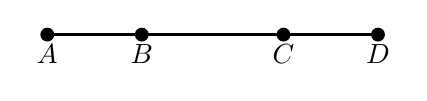
\begin{tikzpicture}\draw[very thick] (0,0)--(4.2,0); \foreach \x/\l in {0/A,1.2/B,3/C,4.2/D} \fill (\x,0) circle(2.5pt) node[below]{$\l$};\end{tikzpicture}\end{center}
Given: $AB = CD$ \qquad Prove: $AC = BD$\par\vspace{1mm}
\renewcommand{\arraystretch}{1.7}\begin{tabular}{@{}l|l@{}}
\textbf{Statements} & \textbf{Reasons}\\ \hline
1.\ $AB = CD$ & Given\\
2.\ $BC = BC$ & \fb[4cm]{Reflexive Property}\\
3.\ $AB + BC = BC + CD$ & \fb[6cm]{Addition Property of Equality}\\
4.\ $AB + BC = AC$, \ $BC + CD = BD$ & \fb[6cm]{Segment Addition Postulate}\\
5.\ $AC = BD$ & \fb[4cm]{Substitution Property}\\
\end{tabular}\end{watchme}

\vid{Watch out}
\begin{mistakebox}A reason must be a \textbf{given}, a \textbf{definition}, a \textbf{property}, a \textbf{postulate} or a \textbf{theorem} --- never ``it \fb[2.4cm]{looks like it}'' or ``I \fb[2.2cm]{calculated it}''.\end{mistakebox}

\vid{Your turn}
\begin{yourturn}Given: $5x - 2 = 18$ \qquad Prove: $x = 4$\par\vspace{1mm}
\renewcommand{\arraystretch}{1.7}\begin{tabular}{@{}l|l@{}}
1.\ $5x - 2 = 18$ & Given\\
2.\ $5x = 20$ & \fb[6cm]{Addition Property of Equality}\\
3.\ $x = 4$ & \fb[6cm]{Division Property of Equality}\\
\end{tabular}\end{yourturn}

\begin{notebox}\textbf{Remember:}\quad \textbf{Statements} on the left, \textbf{reasons} on the right.\quad Start with the \textbf{given}; end with what you must \textbf{prove}.\quad Every reason is a given, definition, property, postulate or theorem.\end{notebox}
\end{document}
